\documentclass{article}
\usepackage[utf8]{inputenc}
\usepackage{amssymb}

\usepackage{listings}
\usepackage{color}
\usepackage{graphicx} %package to manage images

%New colors defined below
\definecolor{codegreen}{rgb}{0,0.6,0}
\definecolor{codegray}{rgb}{0.5,0.5,0.5}
\definecolor{codepurple}{rgb}{0.58,0,0.82}
\definecolor{backcolour}{rgb}{0.95,0.95,0.92}

%Code listing style named "mystyle"
\lstdefinestyle{mystyle}{
  backgroundcolor=\color{backcolour},   commentstyle=\color{codegreen},
  keywordstyle=\color{magenta},
  numberstyle=\tiny\color{codegray},
  stringstyle=\color{codepurple},
  basicstyle=\footnotesize,
  breakatwhitespace=false,         
  breaklines=false,                 
  captionpos=b,                    
  keepspaces=true,                 
  numbers=left,                    
  numbersep=5pt,                  
  showspaces=false,                
  showstringspaces=false,
  showtabs=false,                  
  tabsize=2
}

%"mystyle" code listing set
\lstset{style=mystyle}

\begin{document}
\centerline{\sc \large EECE 7360 Project 2}
\vspace{.5pc}
\centerline{\sc Garrett Goode and Daniel Hullihen}
\centerline{\it Spring 2017}

\section{Introduction}
The subset sum problem (also referred to as the ``exact knapsack problem'')
is defined below.

\textit{Let A = $\{a_1, ..., a_n\}$ represent some set of integers. Given a sum s, find a subset $A' \subset A$ such that
  $$s = \sum_{i=1}^n a_i, for 1 \le i \le n.$$}
In other words, if we are given a list of numbers and some target sum, find the numbers in the list that
add up to the target sum. 

In this project, we explored the complexity landscape around the subset sum
problem, including subproblems to subset sum, as well as problems of which
which subset sum is itself a subproblem.

\section{Natural Subproblems of Subset Sum}
The subset sum problem can be solved in pseudo-polynomial time, which means
there are subproblems to subset sum that can be solved in polynomial time,
but the ``hardest'' subproblem in subset sum is nevertheless NP-Complete. Due
to this property, it is possible to detect some subproblems to subset
sum and apply a known algorithm that solves the problem in polynomial time.
Some algorithms used for solving subset sum use a divide-and-conquer
approach and identify these subproblems. Subproblems
to subset sum, for example, can have all numbers that have some special
property, or the set of numbers itself has some property that can be
exploited.
This section explores some of the natural subproblems to subset sum. 

\subsection{Sets with a low density}
One metric for describing an instance of subset sum is
the density of the set. The following equation
describes the density of a set.
$$d = n / log_2 max(a_i)$$
where n is the size of the set in quation and $max(a_i)$ is the largest
element in the set.
Lagarias and Odlyzko found that, for sets that have a density less than 0.645,
their ``Algorithm SV'' can solve the instance in polynomial
time \cite{lagarias1985}. One of the steps in their algorithm involves
taking set and perform a transformation in order to apply an
algorithm developed by Lenstra, Lenstra, and Lovasz, which has a time
complexity of $O(n^{12}+n^9(log|f|^3))$ \cite{lenstra1982}. The transformed
problem is one where a short vector e must be found within an integer lattice
L = L(a,M)

\subsection{Sets where all the numbers are coprime to m}
This approach (as well as the prior approach) focus on sets that are finite
cyclic groups, defined as $\mathbb{Z}_m = {0, 1, ..., m-1}$ of order m.
Koiliaris and Xu argue that, given a set $S \subseteq U(\mathbb{Z})_m$, which
describes a set of integers that are coprime to some integer m, finding
the set of all subset sums can be donyge with a time complexity of
$O(min(\sqrt{n}m,m^{5/4})log m log n)$ \cite{koiliaris2016}.
Note that an integer x is
coprime to m if the greatest common denomintor of the two values is 1.
As Koiliaris explains, the method behind the speed-up with this approach
is the ability to partition the set into different subsets such that ``every
such subset is contained in an arithmetic progression of the form
x, 2x, ..., lx''. With this, one can calculate the subset sums very quickly
by scaling l accordingly. These sums can then be added together. This is
only doable if m is a prime number, or if all the numbers are relative prime
to m.

\subsection{Set is a subset of $Z_m$}
Koiliaris and Xu are able to take the previous case and take it a step further,
developing an algorithm that finds all of the subsets of a set S in with a
time complexity of $O(min(\sqrt{n}m,m^{5/4})log^2m)$  \cite{koiliaris2016}.
This is for sets $S \subseteq \mathbb{Z}_m$, which is slightly different from
the previous case in that the elements of the set no longer have to be
coprime to some integer m.
Their algorithm involves recursively computing a partial subset sum
as they work across subsets of the original set.

\subsection{Set size $m \geq l^{1/\alpha}$ and elements are distinct}
Chaimovich, Freiman and Galil found that, if they took the subset sum
problem and restricted it such that $max{a_i | a \epsilon A} \leq l \leq
m^\alpha)$ (where l is some bound and m is the number of variables in the set),
then the instance could be solved with a time complexity of $O(lm^2)$
\cite{chaimovich1989}. One unique
feature of their algorithm is that supports large sets (previous algorithms
could only handle moderately large sets). The main approach in their algorithm
is, assuming $A^*$ is defined as ${S_b | B \subseteq A}$, and $S_b$ is
defined as $\sum_{a_i\epsilon B} a_i$, characterize $A^*$ as ``a small
collection of
arithmetic progressions.'' 

\section{Problems of which Subset Sum is a Natural Subproblem}

We were unable to identify any problems of which Subset sum is a natural subproblem.
However rather than ignore this area of investigation entirely, we chose to explore
similar problems that are close neighbors via transformation in the landscape of common
NP-complete problems.

\subsection{Satisfiability} 

While Satisfiability (SAT) is a few transformations away from Subset Sum on the 
complexity landscape we have presented, establishing this link between subset sum and SAT is
crucial as almost all NP completeness proofs are derived from Cook's original proof for SAT and
some transformations. The problem is defined below.

\textit{Given a set of U variables, collection of C clauses over U, is there a satisfying truth assignment for C?}

As proven by Cook in the aforementioned paper, SAT is NP-complete.

\subsection{3-Satisfiability}

Transformed from SAT, 3-Satisfiability (3SAT) is a special case of SAT where each logical 
clause can have only exactly three variables. The problem is formally defined as follows.

\textit{Given a set of U variables, collection of C clauses over U such that $|c| = 3$, is there a satisfying truth assignment for C?}

Despite this restriction on the domain of problem instances when compared to SAT, 
3SAT remains NP-complete.

\subsection{3-Dimensional Matching} 

Transformed from 3SAT, the 3-dimensional matching problem deals with finding a matching in 
a three-dimensional graph. The formal definition is given below.

\textit{Given a set $M \subset WxXxY$, where W, X, and Y are disjoint sets with the same number of elements q, does M contain a matching $M' \subset M$ such that $|M'|= q$ and no two elements are the same?}

Like the previous problems discussed in this section, 3DM remaings NP-complete in all but a few ideal scenarios.
Interestingly enough, 2-Dimensional Matching (2DM) which is not discussed at length in this seciton, is tractable.

\subsection{Partition} 

The Partition problem is defined below.

\textit{Let A = $\{a_1, ..., a_n\}$ represent some set of positive integers. Does there exist a subset $A' \subset A$ such that
  $$\sum_{a \epsilon A'} s(a) = \sum_{a \epsilon A - A'} s(a)?$$}
In other words, is there a subset of the given set with sum equal to the sum of the members of the original set not included in the subset?

Once again, the partition problem is known to be NP-Complete. Of all of the problems discussed in this section,
the partition problem is likely the closest to the Subset Sum problem. However it is not a natural subproblem of Subset Sum
as no target is given as input. Instead, the target is implied as the half of the sum of the input set.

One can see clearly how simple a transformation from an instance of Partition to and instance of Subset Sum would be however, simply
by summing the input set and setting the target total to half of the calculated sum.

\subsection{Knapsack}

The Knapsack problem is also a transformation from the Partition problem (like Subset Sum). As one might expect, the problems are
therefore very similar in nature. The Knapsack problem is defined as follows.

\textit{Given a finite set U, with each $u \epsilon U$ having an associated size s(u) and value v(u), is there a subset $U' \subset U$ such that the sum of the s(u') for all $u' \epsilon U'$ is less than a given integer K while the sum of v(u') for all  $u' \epsilon U'$ is greater than a given integer H?}

Like all of the other problems in this section, knapsack is NP-complete. There are variations of the the Knapsack problem that are
tractable, but they are not discussed in this paper as they are less related to the Subset Sum problem in question. Subset Sum itself
is sometimes refered to as the exact knapsack problem.

\section{Summary}

The chart in Figure 1 on the following page maps out all problems discussed in the preceding sections. Note that all subproblems are tractable, while all problems related by
transformation are believed to be intractable.

\begin{figure}[h]
\centering
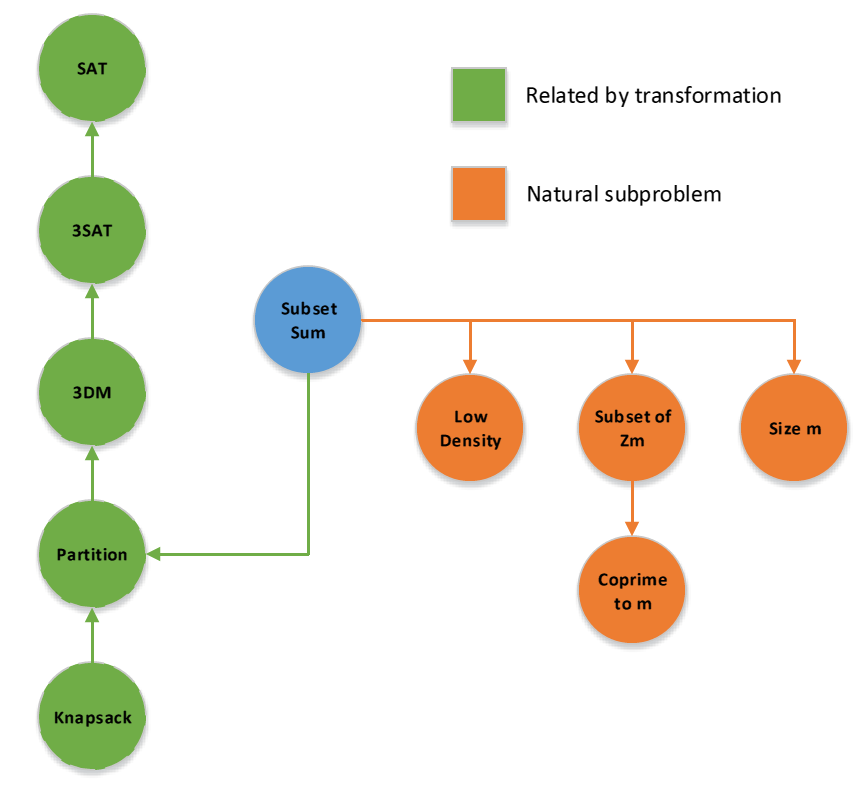
\includegraphics[width=12cm]{comp_chart.png}
\caption{Complexity landscape for Subset Sum}
\end{figure}

\section{Conclusion}

Overall the investigation into the subproblems and closely related NPC problems was very helpful in getting a clearer vision of
the nature of the Subset Sum problem we will continue to investigate. We had some difficulty identifying any problems that
subset sum was a natural subproblem of, but in the end that seemed to be apporpriate as the subset sum problem itself is very general.
It is quite simple to see how when bounds and restrictions are introduced to the origional subset sum problem statement we arrive at
various other important or interesting subproblems, but it is difficult to relax the input domain of a problem that is already so
broad and nonspecific in nature. All in all we are eager to apply the infomation we discovered in this investigation to aid in our
understanding of future solution methods for the Subset Sum problem.

\bibliography{references}
\bibliographystyle{plain}

\end{document}

